\documentclass[11pt]{article}

\usepackage[margin=1in]{geometry}
\usepackage{amsmath,amssymb}
\usepackage{booktabs}
\usepackage{array}
\usepackage{graphicx}
\usepackage{float}
\usepackage{tikz}
\usetikzlibrary{positioning, arrows.meta}
\usepackage[hidelinks]{hyperref}
\graphicspath{{reports/}{./}}

\tikzset{
  box/.style={draw, rounded corners, minimum height=8mm, minimum width=15mm, font=\small},
  noise/.style={draw, dashed, rounded corners, minimum height=7mm, font=\footnotesize\itshape},
  >=Stealth,
}

\title{Engression on Real ENA Weather Data: A Brief Summary}
\author{WeatherEngression Research Notes}
\date{\today}

\begin{document}
\maketitle

\section{Model Architectures}

All models learn a conditional sampler \(\widehat{Y}=g(X,\varepsilon)\) with fresh
noise \(\varepsilon\) per draw, trained with the energy-score (CRPS) loss; repeated
draws approximate \(P(Y\mid X)\). They differ in how \(X\) is read and where
\(\varepsilon\) enters.

\begin{itemize}
  \item \textbf{Built-in (vanilla).} The public \texttt{engression} model: \(X\) is
  flattened and fed to a StoNet (MLP with fresh noise concatenated at every layer).
  No time order.
  \item \textbf{LSTM + default head.} LSTM encoder \(\to\) summary \(h(X)\); one
  noise vector concatenated to \(h(X)\), then a plain MLP.
  \(\widehat{Y}=g(h(X),\varepsilon)\).
  \item \textbf{LSTM + StoNet head.} Same encoder; the head re-injects noise at
  every layer. No monotonicity.
  \item \textbf{LSTM + pre-additive head.} \(Y=g(\phi(X)+\eta)\): the encoder makes
  a low-dimensional index \(\phi(X)\), noise \(\eta\) is \emph{added}, and a
  monotone \(g\) maps to the target. The only head with the paper's extrapolation
  theory.
\end{itemize}

\noindent
Noise enters late, after a deterministic encoder: the uncertainty is in the scalar
target, and noise injected deep into a 241-step recurrence tends to be forgotten.

\begin{figure}[H]
  \centering
  % (a) vanilla
  \textbf{(a) Built-in (vanilla)}\\[2pt]
  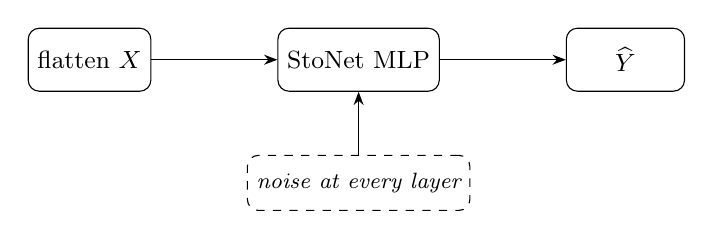
\begin{tikzpicture}[node distance=16mm]
    \node[box] (x) {flatten $X$};
    \node[box, right=of x] (net) {StoNet MLP};
    \node[box, right=of net] (y) {$\widehat{Y}$};
    \node[noise, below=8mm of net] (e) {noise at every layer};
    \draw[->] (x) -- (net);
    \draw[->] (net) -- (y);
    \draw[->] (e) -- (net);
  \end{tikzpicture}\\[10pt]
  % (b) LSTM default
  \textbf{(b) LSTM + default head}\\[2pt]
  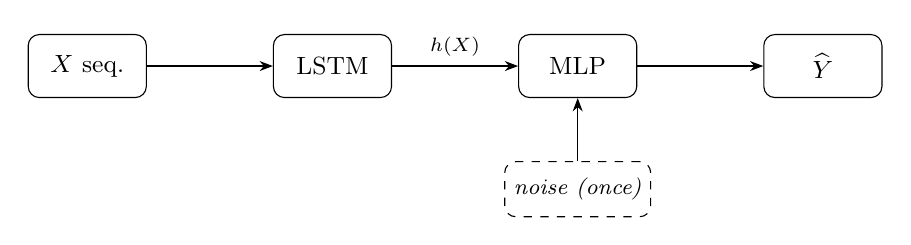
\begin{tikzpicture}[node distance=16mm]
    \node[box] (x) {$X$ seq.};
    \node[box, right=of x] (lstm) {LSTM};
    \node[box, right=of lstm] (mlp) {MLP};
    \node[box, right=of mlp] (y) {$\widehat{Y}$};
    \node[noise, below=8mm of mlp] (e) {noise (once)};
    \draw[->] (x) -- (lstm);
    \draw[->] (lstm) -- node[above, font=\scriptsize] {$h(X)$} (mlp);
    \draw[->] (mlp) -- (y);
    \draw[->] (e) -- (mlp);
  \end{tikzpicture}\\[10pt]
  % (c) LSTM StoNet
  \textbf{(c) LSTM + StoNet head}\\[2pt]
  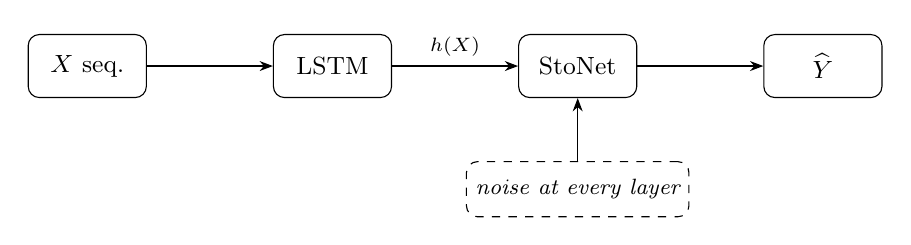
\begin{tikzpicture}[node distance=16mm]
    \node[box] (x) {$X$ seq.};
    \node[box, right=of x] (lstm) {LSTM};
    \node[box, right=of lstm] (net) {StoNet};
    \node[box, right=of net] (y) {$\widehat{Y}$};
    \node[noise, below=8mm of net] (e) {noise at every layer};
    \draw[->] (x) -- (lstm);
    \draw[->] (lstm) -- node[above, font=\scriptsize] {$h(X)$} (net);
    \draw[->] (net) -- (y);
    \draw[->] (e) -- (net);
  \end{tikzpicture}\\[10pt]
  % (d) LSTM pre-additive
  \textbf{(d) LSTM + pre-additive head}\\[2pt]
  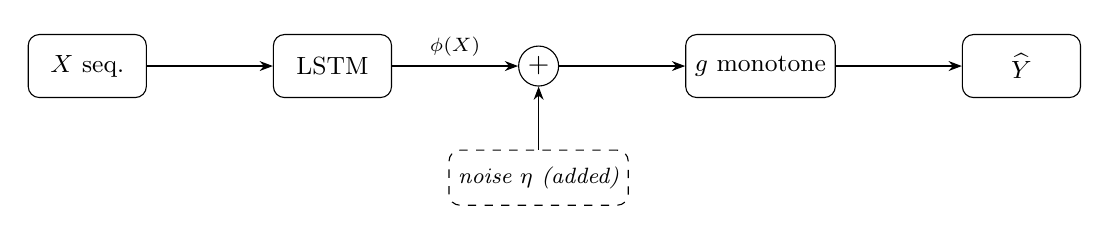
\begin{tikzpicture}[node distance=16mm]
    \node[box] (x) {$X$ seq.};
    \node[box, right=of x] (lstm) {LSTM};
    \node[circle, draw, right=of lstm, inner sep=1.5pt] (plus) {$+$};
    \node[box, right=of plus] (g) {$g$ monotone};
    \node[box, right=of g] (y) {$\widehat{Y}$};
    \node[noise, below=8mm of plus] (e) {noise $\eta$ (added)};
    \draw[->] (x) -- (lstm);
    \draw[->] (lstm) -- node[above, font=\scriptsize] {$\phi(X)$} (plus);
    \draw[->] (plus) -- (g);
    \draw[->] (g) -- (y);
    \draw[->] (e) -- (plus);
  \end{tikzpicture}
  \caption{Data and noise inputs per model. $X$ enters from the left, noise from
  below (dashed). Noise is concatenated in (a)--(c) and added to $\phi(X)$ in (d).}
\end{figure}

\begin{table}[h]
  \centering
  \small
  \caption{Engression assumptions by architecture. \emph{achieved} = holds by
  construction; \emph{hoped} = the structure is present but the guarantee is not
  exact; \emph{violated} = the assumption does not hold.}
  \label{tab:assumptions}
  \begin{tabular}{lcccc}
    \toprule
    Architecture & Learns $P(Y\mid X)$ & Pre-additive noise & Monotone $g$ & Extrapolation theory \\
    \midrule
    Vanilla (flat StoNet) & achieved$^{\dagger}$ & violated & violated & none \\
    LSTM $+$ default head & achieved$^{\dagger}$ & violated & violated & none \\
    LSTM $+$ StoNet head & achieved$^{\dagger}$ & violated & violated & none \\
    LSTM $+$ pre-additive & achieved$^{\dagger}$ & achieved & achieved & hoped$^{\ddagger}$ \\
    \bottomrule
  \end{tabular}

  \smallskip
  {\footnotesize $^{\dagger}$ targeted by the energy loss; achieved \emph{in
  practice} only when the noise channel does not collapse (the under-dispersion of
  Section~\ref{sec:insample}).\quad
  $^{\ddagger}$ the pre-additive form and a monotone $g$ are present, but the index
  $\phi(X)=W\!\cdot\!\mathrm{LSTM}(X)$ is \emph{nonlinear}, whereas the paper's
  extrapolation theorem assumes a \emph{linear} index---so the guarantee is hoped
  for, not proven.}
\end{table}

\section{Experimental Setup}

\textbf{Data.} Eastern North Atlantic (ENA) observations. Each sample is a
$10$-day airmass back-trajectory of $241$ hourly time steps $\times$ $22$ weather
variables; the target is $\log_{10}(\mathrm{CCN})$, the cloud-condensation-nuclei
concentration at arrival. After dropping samples with a missing target there are
$\approx 60{,}866$ usable trajectories.

\medskip
\noindent
\textbf{Train/test split (``paper'' split).} Six alternating months of 2022 (Jan,
Mar, May, Jul, Sep, Nov) are the test set; all other months train. Whole-month
blocks prevent autocorrelated neighbouring hours from leaking across the split.
This gives $57{,}646$ training and $3{,}220$ test trajectories. Since the held-out
months are interleaved with training months, this is \emph{in-distribution /
interpolation}, not extrapolation.

\medskip
\noindent
\textbf{Dimensions.} The LSTM keeps the unflattened sequence,
$X\in\mathbb{R}^{57646\times 241\times 22}$ (train). The flat (vanilla) model
instead flattens each trajectory to $241\times 22 = 5302$ features.

\section{In-Sample Performance}
\label{sec:insample}

We score the predictive distribution against the held-out (in-distribution)
targets with: 90\% interval coverage (nominal $0.90$; closer is better),
interval width (smaller = sharper), median absolute error (MAE), and the energy
score / CRPS (lower = better distributional fit).

Our primary model is the \textbf{LSTM + StoNet head}; Table~\ref{tab:stonet} is its
full sweep, and Table~\ref{tab:preadd} the pre-additive head for comparison.

\begin{table}[h]
  \centering
  \caption{\textbf{LSTM + StoNet head} (primary model): full $8$-configuration
  sweep, sorted by CRPS. Lower width / MAE / CRPS is better; coverage near $0.90$ is
  better. Starred row ($\star$): recommended configuration (Figures~\ref{fig:bands},
  \ref{fig:oos}).}
  \label{tab:stonet}
  \begin{tabular}{rrr ccccc}
    \toprule
    lr & depth & hidden & cov.\ 90\% & cov.\ 50\% & width & MAE & CRPS \\
    \midrule
    $0.003$ & $5$ & $192$ & $0.783$ & $0.378$ & $0.50$ & $0.164$ & $0.120$ \\
    $\star$\,$0.01$ & $5$ & $128$ & $\mathbf{0.844}$ & $\mathbf{0.438}$ & $\mathbf{0.65}$ & $\mathbf{0.171}$ & $\mathbf{0.123}$ \\
    $0.003$ & $5$ & $128$ & $0.573$ & $0.241$ & $0.34$ & $0.176$ & $0.137$ \\
    $0.003$ & $3$ & $128$ & $0.458$ & $0.206$ & $0.26$ & $0.176$ & $0.143$ \\
    $0.003$ & $3$ & $192$ & $0.384$ & $0.158$ & $0.22$ & $0.180$ & $0.151$ \\
    $0.01$  & $3$ & $128$ & $0.907$ & $0.505$ & $0.97$ & $0.212$ & $0.152$ \\
    $0.01$  & $5$ & $192$ & $0.762$ & $0.488$ & $0.79$ & $0.216$ & $0.161$ \\
    $0.01$  & $3$ & $192$ & $0.856$ & $0.310$ & $0.86$ & $0.226$ & $0.166$ \\
    \bottomrule
  \end{tabular}
\end{table}

\begin{table}[h]
  \centering
  \caption{\textbf{LSTM + pre-additive head}, for comparison. Depth is set by a
  separate monotone-net parameter, so \texttt{num\_layer} had no effect; the four
  distinct configurations are shown. Uniformly weaker than StoNet.}
  \label{tab:preadd}
  \begin{tabular}{rr ccccc}
    \toprule
    lr & hidden & cov.\ 90\% & cov.\ 50\% & width & MAE & CRPS \\
    \midrule
    $0.003$ & $128$ & $0.386$ & $0.162$ & $0.22$ & $0.186$ & $0.157$ \\
    $0.003$ & $192$ & $0.321$ & $0.133$ & $0.18$ & $0.182$ & $0.157$ \\
    $0.01$  & $128$ & $0.838$ & $0.450$ & $0.86$ & $0.233$ & $0.168$ \\
    $0.01$  & $192$ & $0.511$ & $0.216$ & $0.62$ & $0.388$ & $0.311$ \\
    \bottomrule
  \end{tabular}
\end{table}

\begin{table}[h]
  \centering
  \caption{\textbf{LSTM + default head} (unconstrained MLP). A single full-data run,
  \emph{not} swept --- the baseline referenced below. Best raw CRPS, but lacks the
  pre-additive structure.}
  \label{tab:default}
  \begin{tabular}{rrr ccccc}
    \toprule
    lr & depth & hidden & cov.\ 90\% & cov.\ 50\% & width & MAE & CRPS \\
    \midrule
    $0.003$ & $3$ & $192$ & $0.888$ & $0.480$ & $0.69$ & $0.176$ & $0.126$ \\
    \bottomrule
  \end{tabular}
\end{table}

\begin{table}[H]
  \centering
  \small
  \caption{\textbf{Vanilla (flat) baseline}: full $24$-configuration sweep, sorted by
  CRPS. Starred row ($\star$): the config shown in Figure~\ref{fig:bands} (highest
  coverage). The pattern is the flat model's whole story: the lowest-CRPS configs are
  sharp but badly \emph{under}-cover ($\sim0.3$--$0.5$), and the only configs that
  reach $\sim0.9$ coverage (lr $0.01$, depth $5$) do so with the \emph{widest}, least
  accurate intervals --- it covers only by hedging.}
  \label{tab:vanilla}
  \begin{tabular}{rrrr ccccc}
    \toprule
    lr & depth & hidden & noise & cov.\ 90\% & cov.\ 50\% & width & MAE & CRPS \\
    \midrule
    $0.003$ & $3$ & $256$ & $64$ & $0.392$ & $0.174$ & $0.21$ & $0.167$ & $0.139$ \\
    $0.003$ & $3$ & $256$ & $128$ & $0.416$ & $0.177$ & $0.24$ & $0.173$ & $0.142$ \\
    $0.01$ & $3$ & $128$ & $64$ & $0.536$ & $0.246$ & $0.33$ & $0.183$ & $0.144$ \\
    $0.003$ & $3$ & $128$ & $64$ & $0.426$ & $0.183$ & $0.24$ & $0.177$ & $0.145$ \\
    $0.01$ & $3$ & $256$ & $128$ & $0.539$ & $0.233$ & $0.34$ & $0.189$ & $0.148$ \\
    $0.001$ & $3$ & $256$ & $128$ & $0.304$ & $0.121$ & $0.17$ & $0.172$ & $0.148$ \\
    $0.003$ & $3$ & $128$ & $128$ & $0.398$ & $0.172$ & $0.24$ & $0.181$ & $0.149$ \\
    $0.01$ & $3$ & $256$ & $64$ & $0.421$ & $0.185$ & $0.27$ & $0.184$ & $0.149$ \\
    $0.001$ & $3$ & $256$ & $64$ & $0.310$ & $0.132$ & $0.18$ & $0.174$ & $0.149$ \\
    $0.01$ & $3$ & $128$ & $128$ & $0.532$ & $0.238$ & $0.39$ & $0.195$ & $0.151$ \\
    $0.003$ & $5$ & $128$ & $128$ & $0.379$ & $0.150$ & $0.23$ & $0.183$ & $0.152$ \\
    $0.001$ & $5$ & $256$ & $64$ & $0.268$ & $0.103$ & $0.15$ & $0.175$ & $0.153$ \\
    $0.001$ & $5$ & $256$ & $128$ & $0.263$ & $0.107$ & $0.15$ & $0.177$ & $0.154$ \\
    $0.003$ & $5$ & $256$ & $64$ & $0.273$ & $0.107$ & $0.16$ & $0.179$ & $0.155$ \\
    $0.001$ & $3$ & $128$ & $64$ & $0.289$ & $0.118$ & $0.18$ & $0.180$ & $0.155$ \\
    $0.001$ & $5$ & $128$ & $64$ & $0.290$ & $0.123$ & $0.17$ & $0.179$ & $0.155$ \\
    $0.001$ & $3$ & $128$ & $128$ & $0.287$ & $0.118$ & $0.17$ & $0.180$ & $0.156$ \\
    $0.003$ & $5$ & $256$ & $128$ & $0.287$ & $0.112$ & $0.16$ & $0.180$ & $0.156$ \\
    $0.003$ & $5$ & $128$ & $64$ & $0.311$ & $0.118$ & $0.18$ & $0.184$ & $0.158$ \\
    $0.001$ & $5$ & $128$ & $128$ & $0.295$ & $0.125$ & $0.17$ & $0.182$ & $0.158$ \\
    $\star$\,$0.01$ & $5$ & $128$ & $64$ & $0.907$ & $0.487$ & $1.02$ & $0.227$ & $0.162$ \\
    $0.01$ & $5$ & $128$ & $128$ & $0.924$ & $0.514$ & $1.09$ & $0.227$ & $0.162$ \\
    $0.01$ & $5$ & $256$ & $64$ & $0.850$ & $0.420$ & $0.84$ & $0.227$ & $0.163$ \\
    $0.01$ & $5$ & $256$ & $128$ & $0.461$ & $0.071$ & $0.53$ & $0.227$ & $0.200$ \\
    \bottomrule
  \end{tabular}
\end{table}

\noindent
\textbf{Baselines (context only).} The flat \emph{vanilla} model (Table~\ref{tab:vanilla})
reached coverage $0.907$ only by widening (width $1.02$, MAE $0.227$, CRPS $0.162$) ---
its best CRPS ($0.139$) comes from a sharp config that under-covers at $0.39$. The
unconstrained LSTM\,$+$\,MLP head (Table~\ref{tab:default}) reaches CRPS $0.126$, below
every vanilla config; we report StoNet as the constrained engression head.

\begin{figure}[H]
  \centering
  \begin{minipage}{0.49\textwidth}\centering
    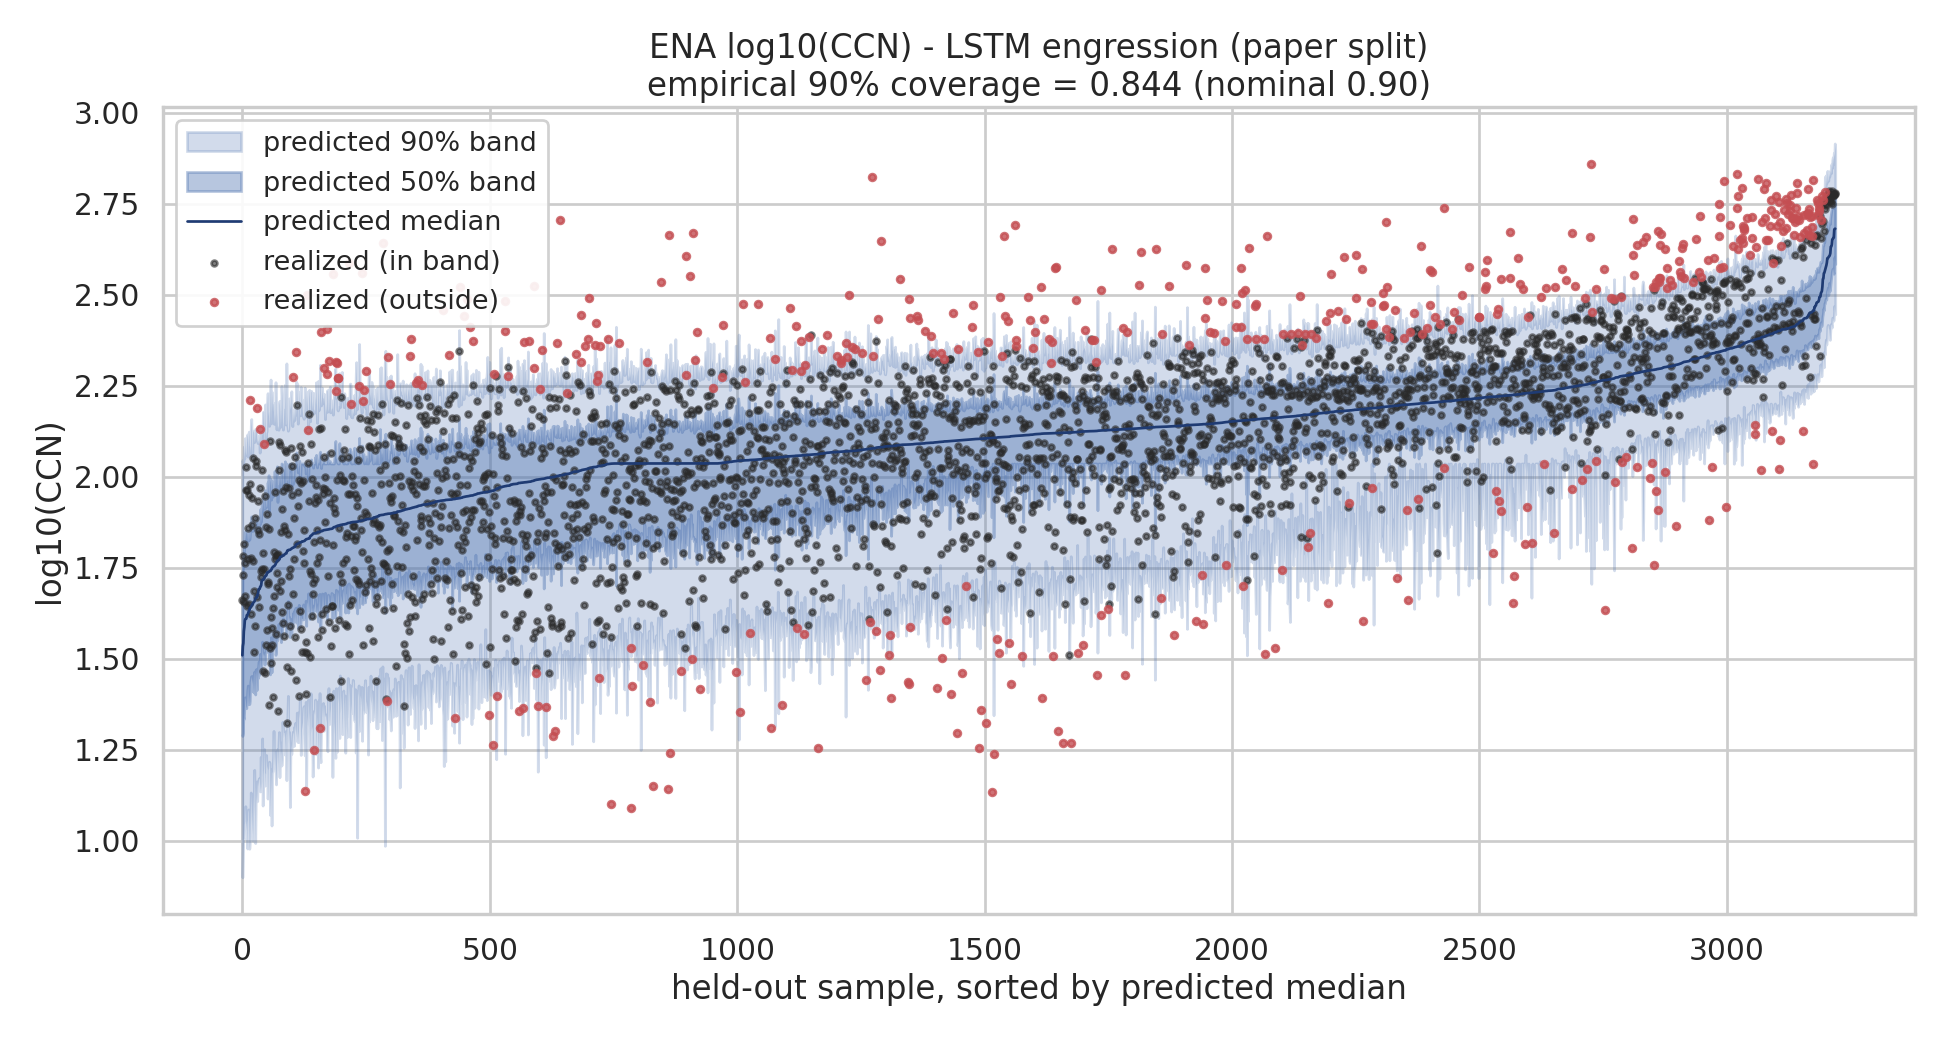
\includegraphics[width=\textwidth]{fig_stonet_is.png}\\[-0.2em]
    {\small \textbf{StoNet} ($5\times128$): cov.\ $0.844$}
  \end{minipage}\hfill
  \begin{minipage}{0.49\textwidth}\centering
    \IfFileExists{reports/fig_default_is.png}
      {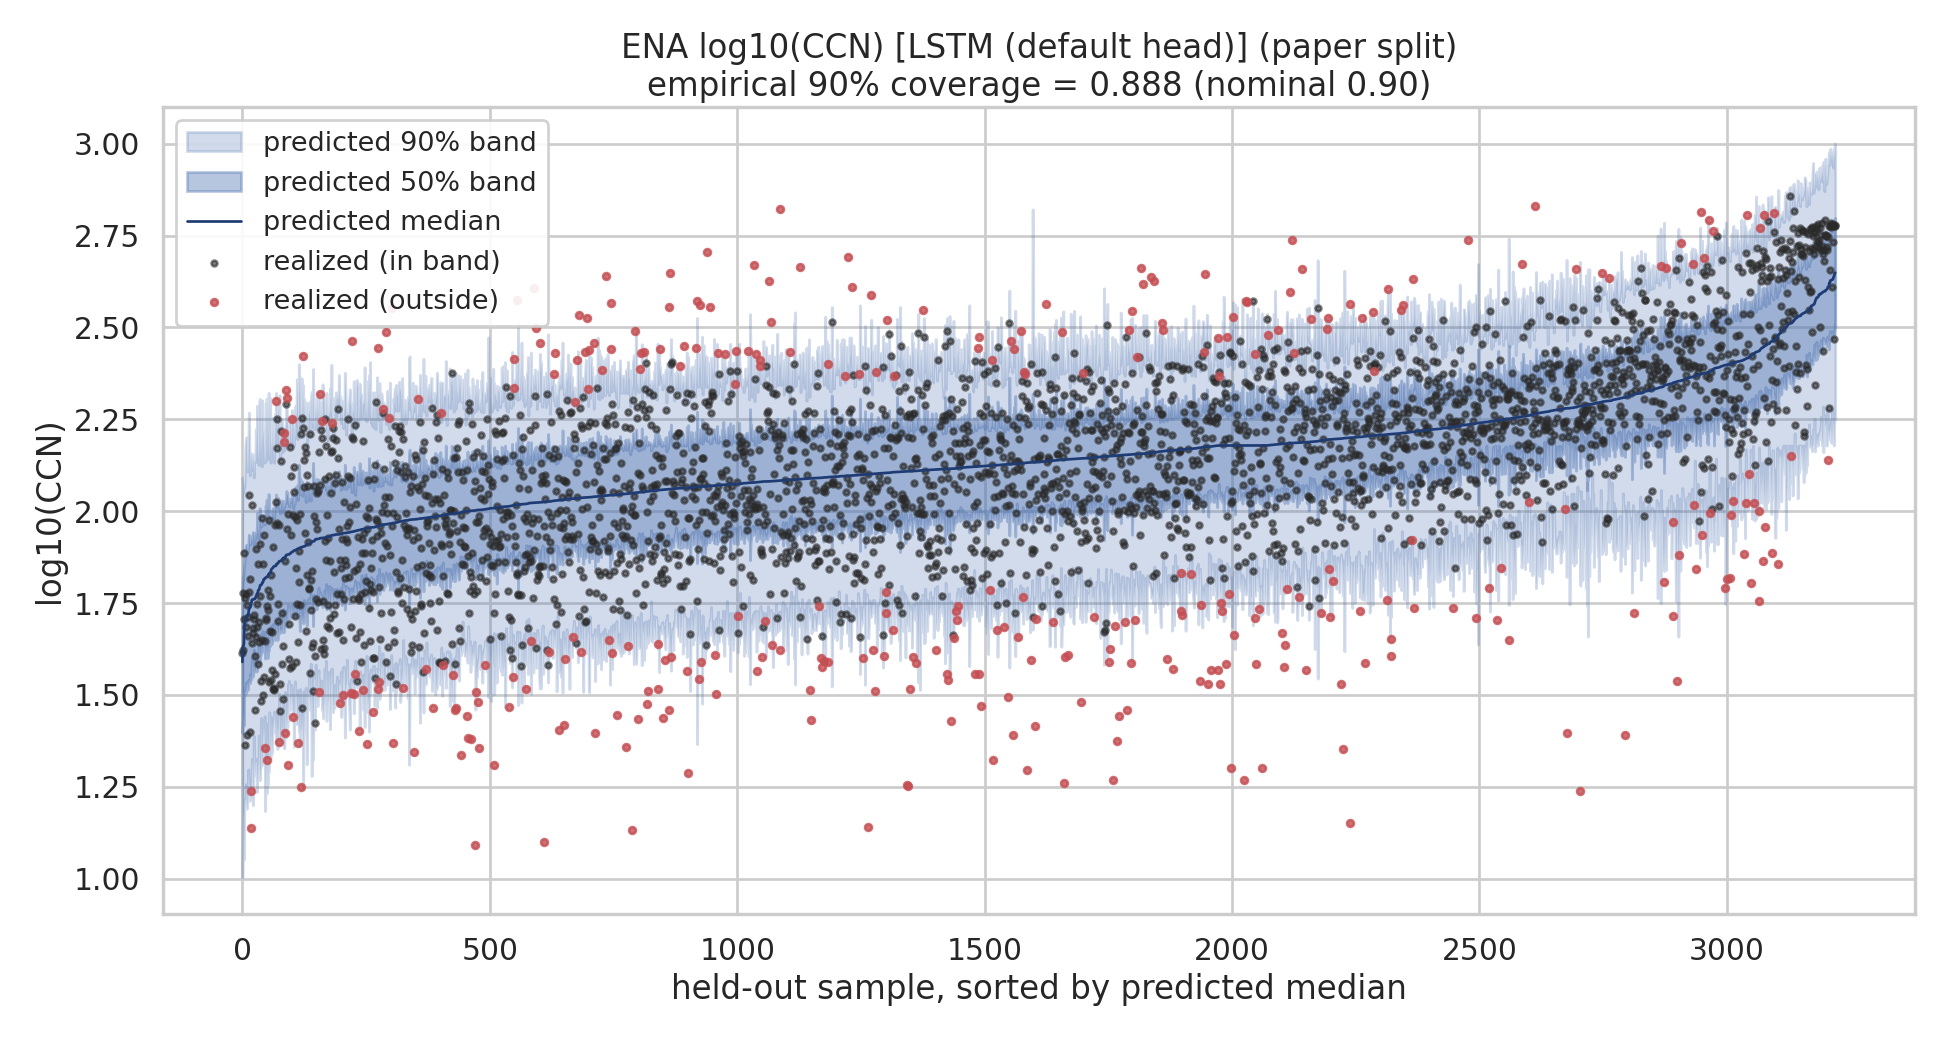
\includegraphics[width=\textwidth]{fig_default_is.png}}
      {\fbox{\parbox[c][3.0cm][c]{0.9\textwidth}{\centering\small default-head chart\\pending GPU rerun\\(\texttt{slurm/regen\_default\_charts})}}}
    \\[-0.2em]{\small \textbf{Default head} ($3\times192$): cov.\ $0.888$}
  \end{minipage}
  \\[6pt]
  \begin{minipage}{0.49\textwidth}\centering
    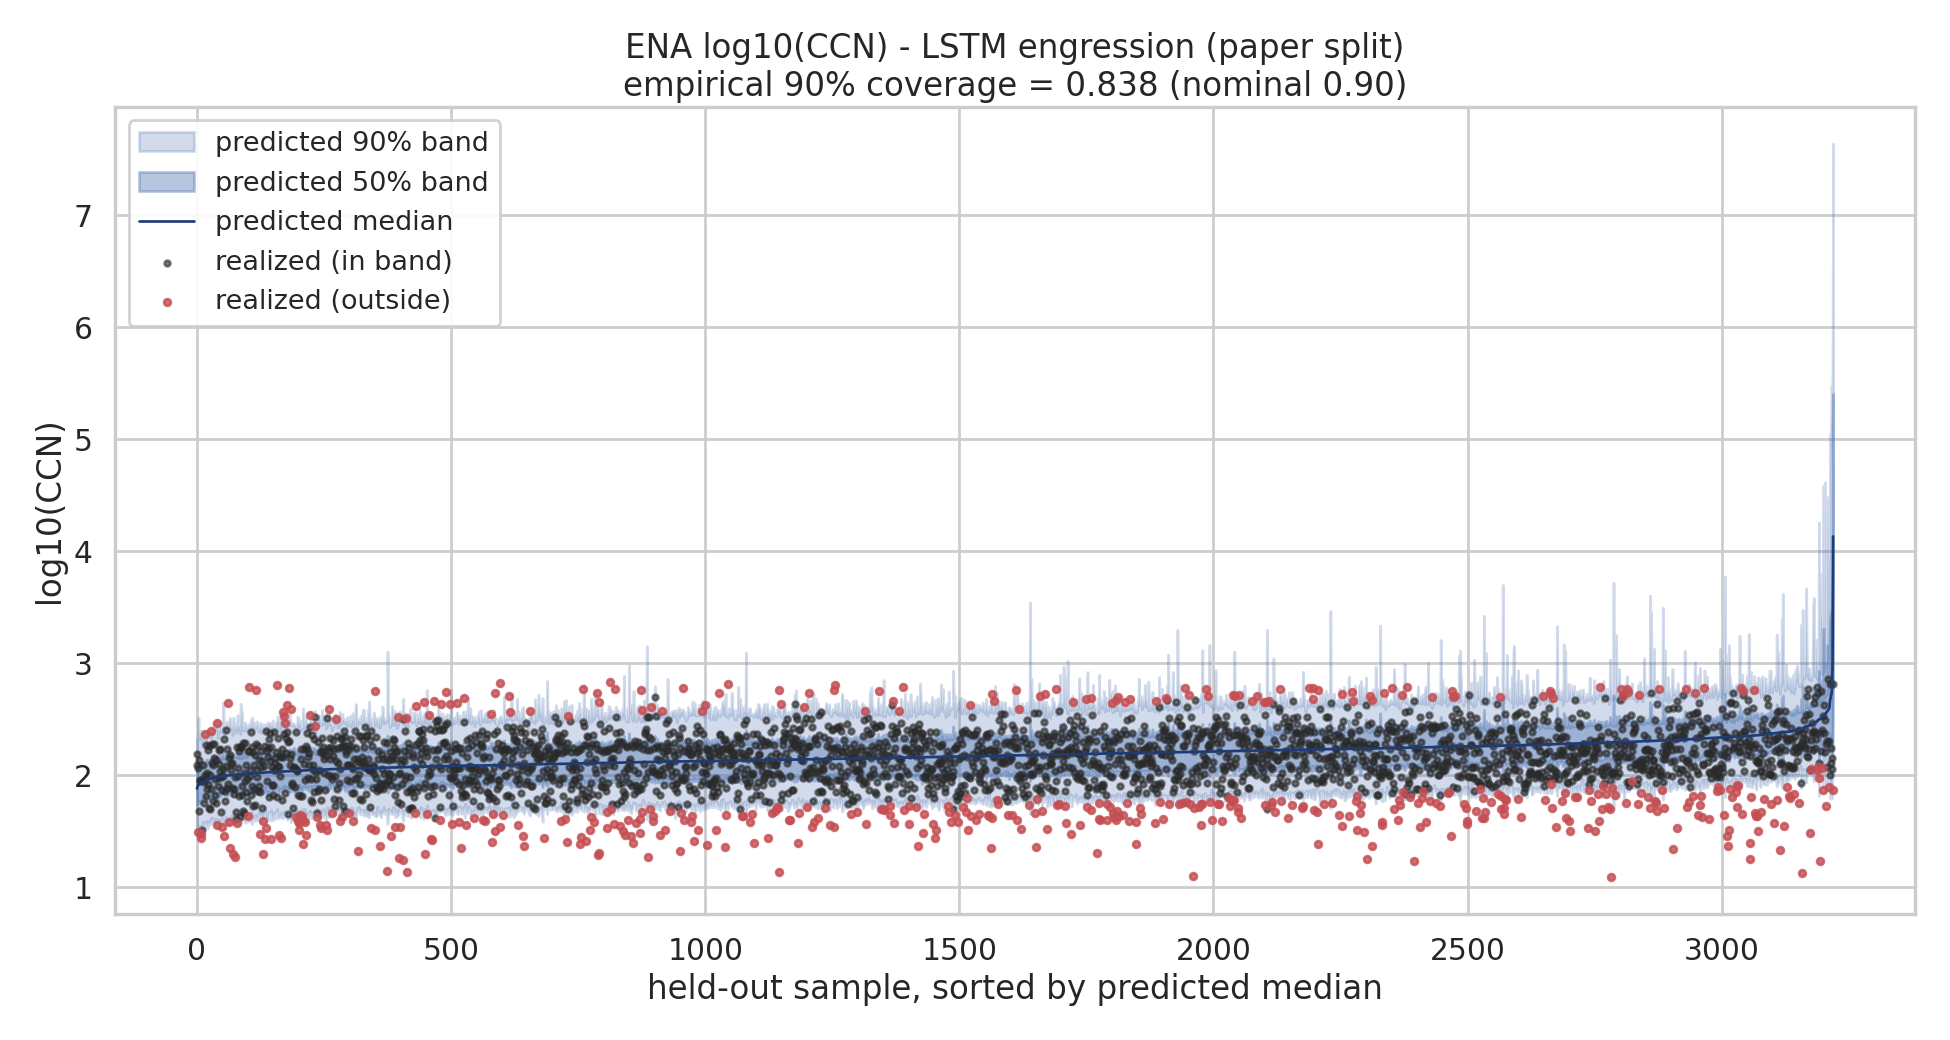
\includegraphics[width=\textwidth]{fig_preadd_is.png}\\[-0.2em]
    {\small \textbf{Pre-additive} (hidden 128): cov.\ $0.838$}
  \end{minipage}\hfill
  \begin{minipage}{0.49\textwidth}\centering
    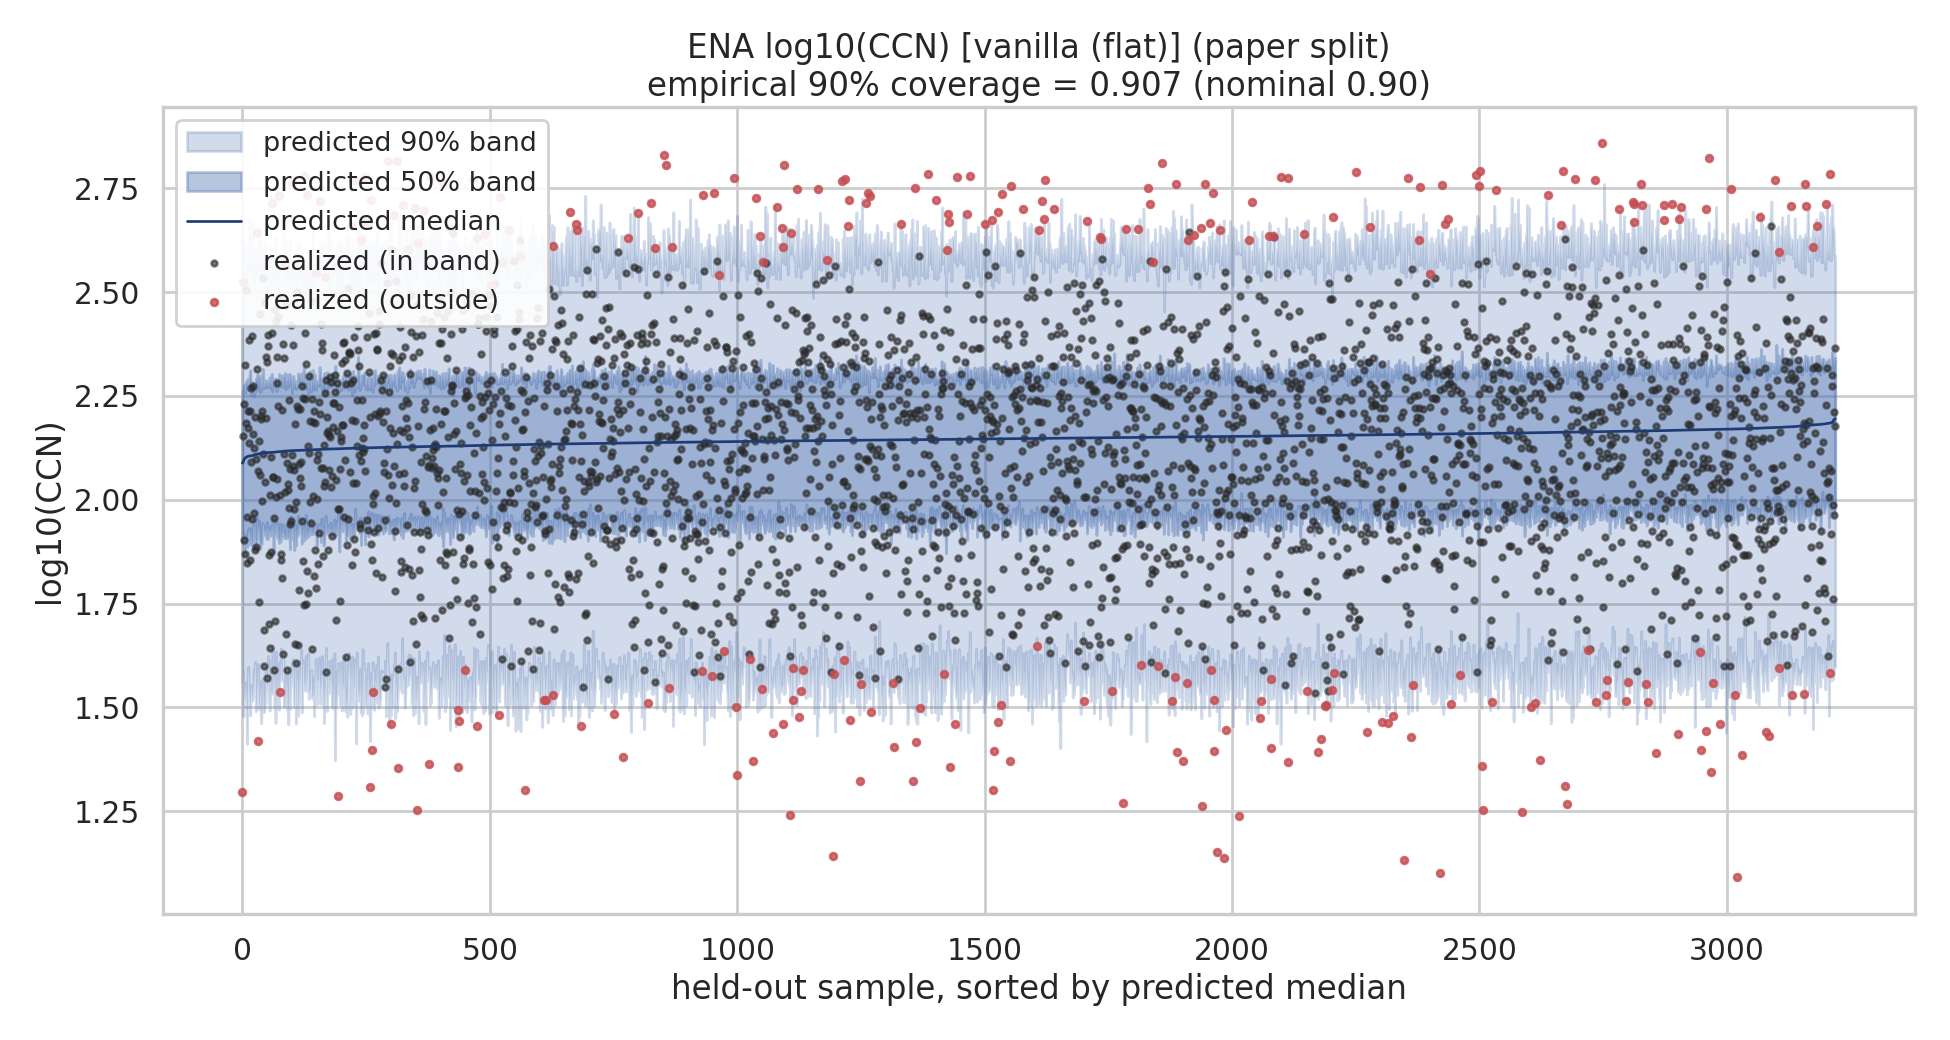
\includegraphics[width=\textwidth]{fig_vanilla_is.png}\\[-0.2em]
    {\small \textbf{Vanilla (flat)} ($5\times128$): cov.\ $0.907$}
  \end{minipage}
  \caption{In-sample posterior bands for each architecture's best run. Points sorted
  by predicted median; shaded bands are the predicted 50\% and 90\% intervals; dots
  are realised $\log_{10}(\mathrm{CCN})$ (red $=$ outside the 90\% band).}
  \label{fig:bands}
\end{figure}

\paragraph{Sweep details.} Tables~\ref{tab:stonet}--\ref{tab:preadd} are the full
LSTM head sweep ($16$ runs: head $\times$ learning rate
$\{0.003,0.01\}$ $\times$ depth $\{3,5\}$ $\times$ hidden
$\{128,192\}$, noise dimension fixed at $96$). The flat (vanilla) baseline was
swept separately over $24$ configurations (learning rate
$\in\{0.001,0.003,0.01\}$, width $\in\{128,256\}$, depth $\in\{3,5\}$,
noise dimension $\in\{64,128\}$). Fixed throughout: $\log_{10}(\mathrm{CCN})$
target, paper split, full data, batch size $256$, weight decay $0$, early stopping
on the training energy loss.

\noindent
\textbf{Takeaways.}
\begin{itemize}
  \item \textbf{Sequence structure helps.} The LSTM is calibrated while staying
  sharp and accurate; the flat model reaches coverage only with wide, inaccurate
  intervals.
  \item \textbf{Under-dispersion is the main failure.} Many configurations collapse
  to a sharp point and lose coverage; coverage \emph{anti-correlates} with
  sharpness.
  \item \textbf{What controls collapse.} Learning rate dominates (StoNet collapsed
  at lr$=0.003$, recovered at lr$=0.01$); more \emph{depth} helps, more \emph{width}
  hurts.
\end{itemize}

\section{Out-of-Sample Performance}

We measure each test point's distance from training in the LSTM embedding space
($k$NN and Mahalanobis), then stratify coverage by it.

\medskip
\noindent
\textbf{Findings.}
\begin{itemize}
  \item Both heads' best runs are roughly \emph{flat} across distance
  (Figure~\ref{fig:oos}): calibration is robust across the training support.
  Under-dispersed (collapsed) configurations instead lose coverage with distance.
  \item $k$NN and Mahalanobis agree closely.
\end{itemize}

\begin{figure}[H]
  \centering
  \begin{minipage}{0.49\textwidth}\centering
    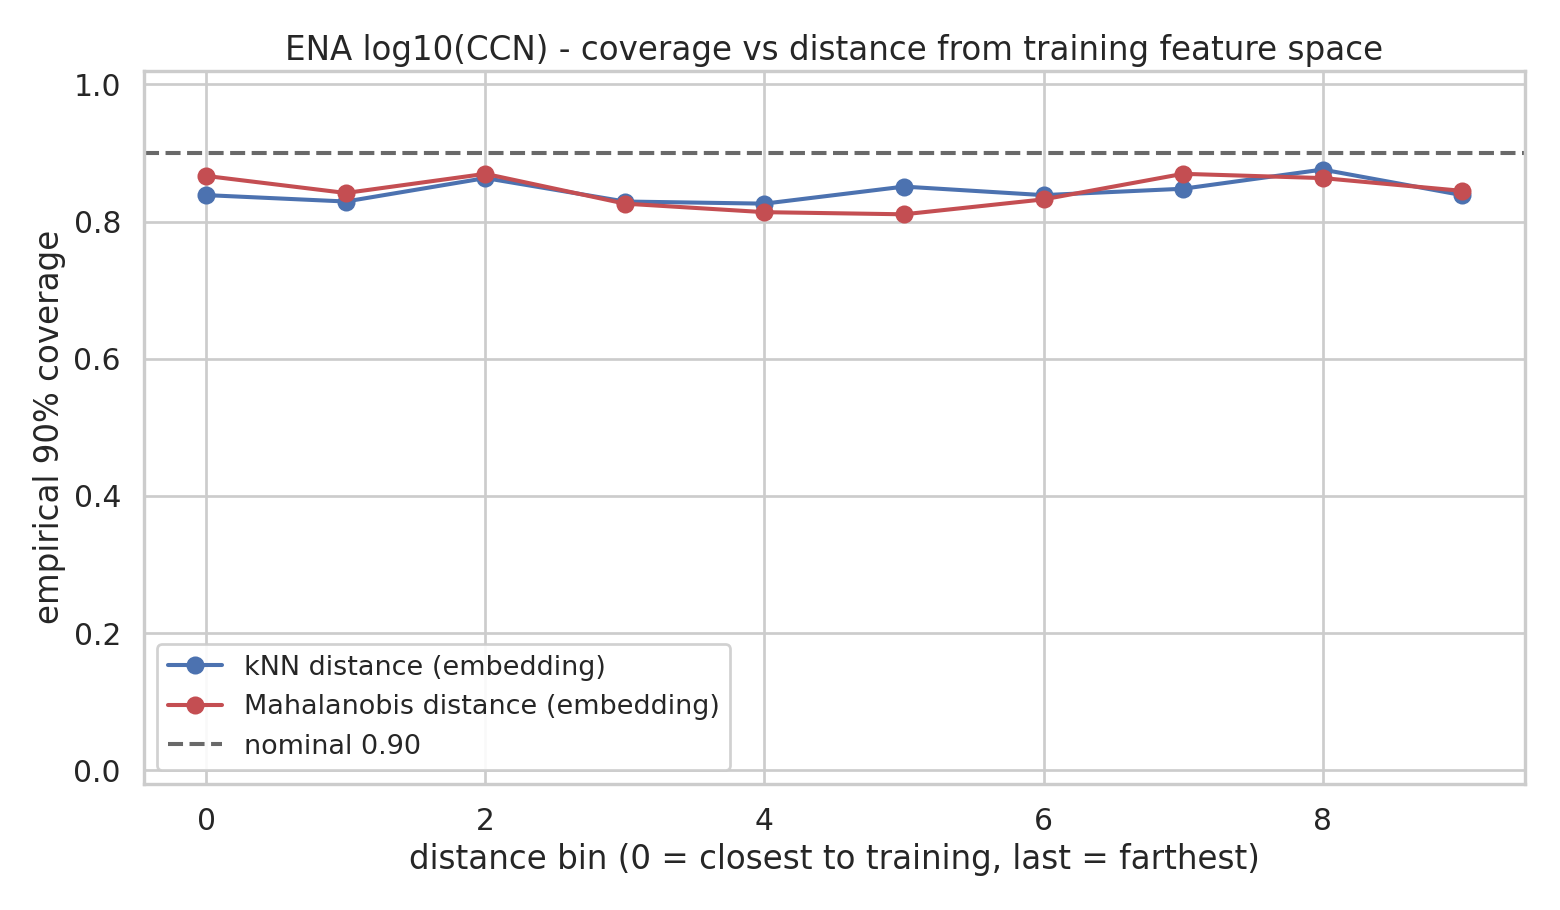
\includegraphics[width=\textwidth]{fig_stonet_oos.png}
    \\[-0.2em]{\small \textbf{StoNet} ($5\times128$)}
  \end{minipage}\hfill
  \begin{minipage}{0.49\textwidth}\centering
    \IfFileExists{reports/fig_default_oos.png}
      {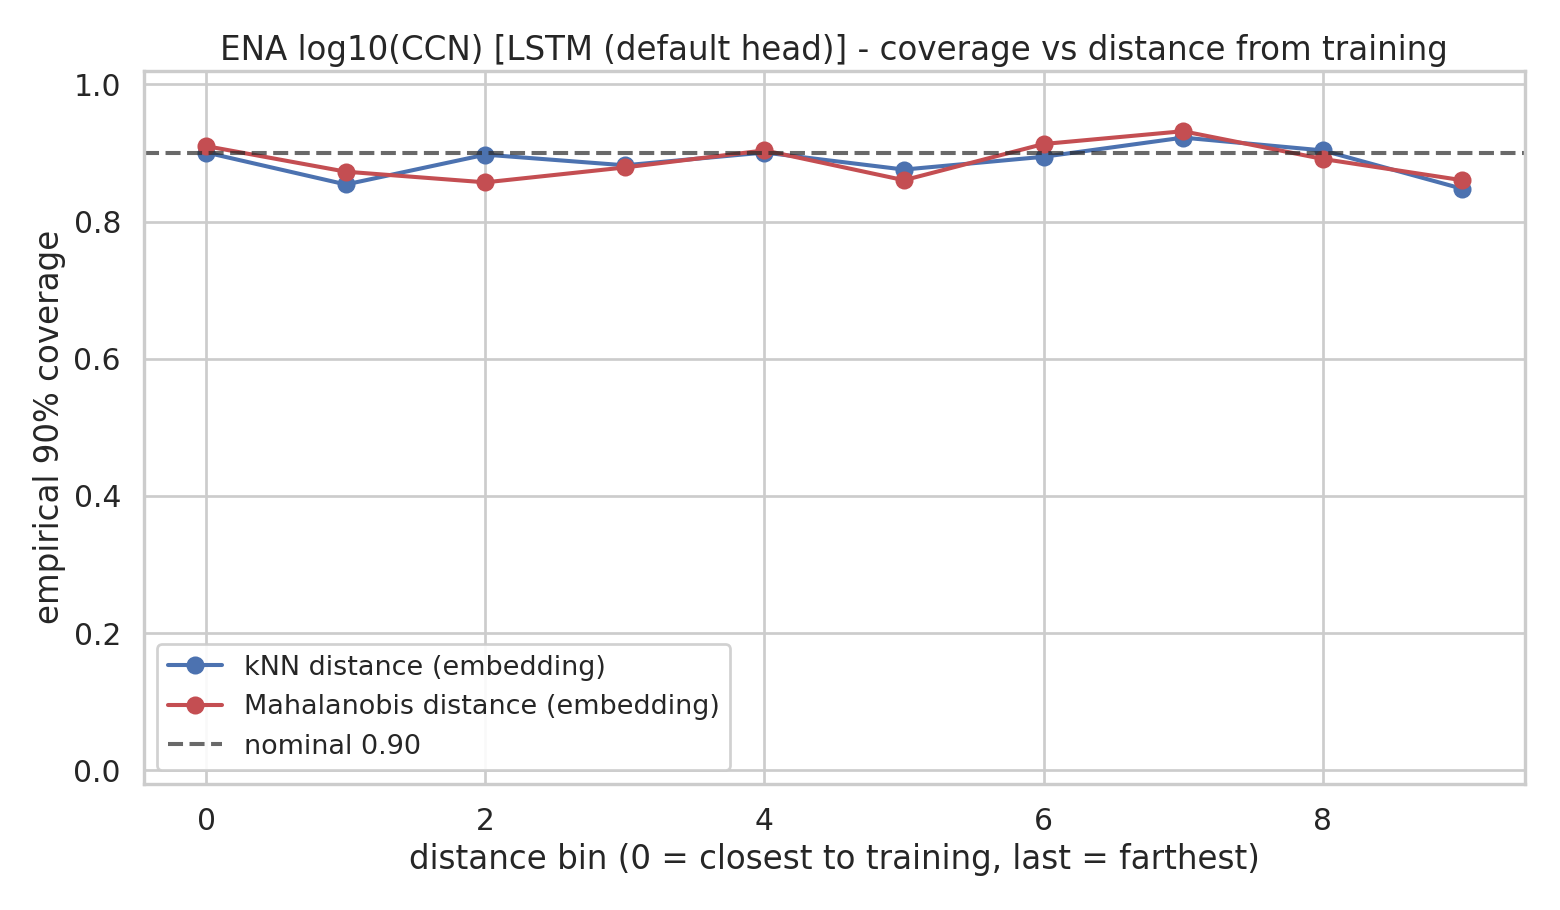
\includegraphics[width=\textwidth]{fig_default_oos.png}}
      {\fbox{\parbox[c][3.0cm][c]{0.9\textwidth}{\centering\small default-head chart\\pending GPU rerun\\(\texttt{slurm/regen\_default\_charts})}}}
    \\[-0.2em]{\small \textbf{Default head} ($3\times192$)}
  \end{minipage}
  \\[6pt]
  \begin{minipage}{0.49\textwidth}\centering
    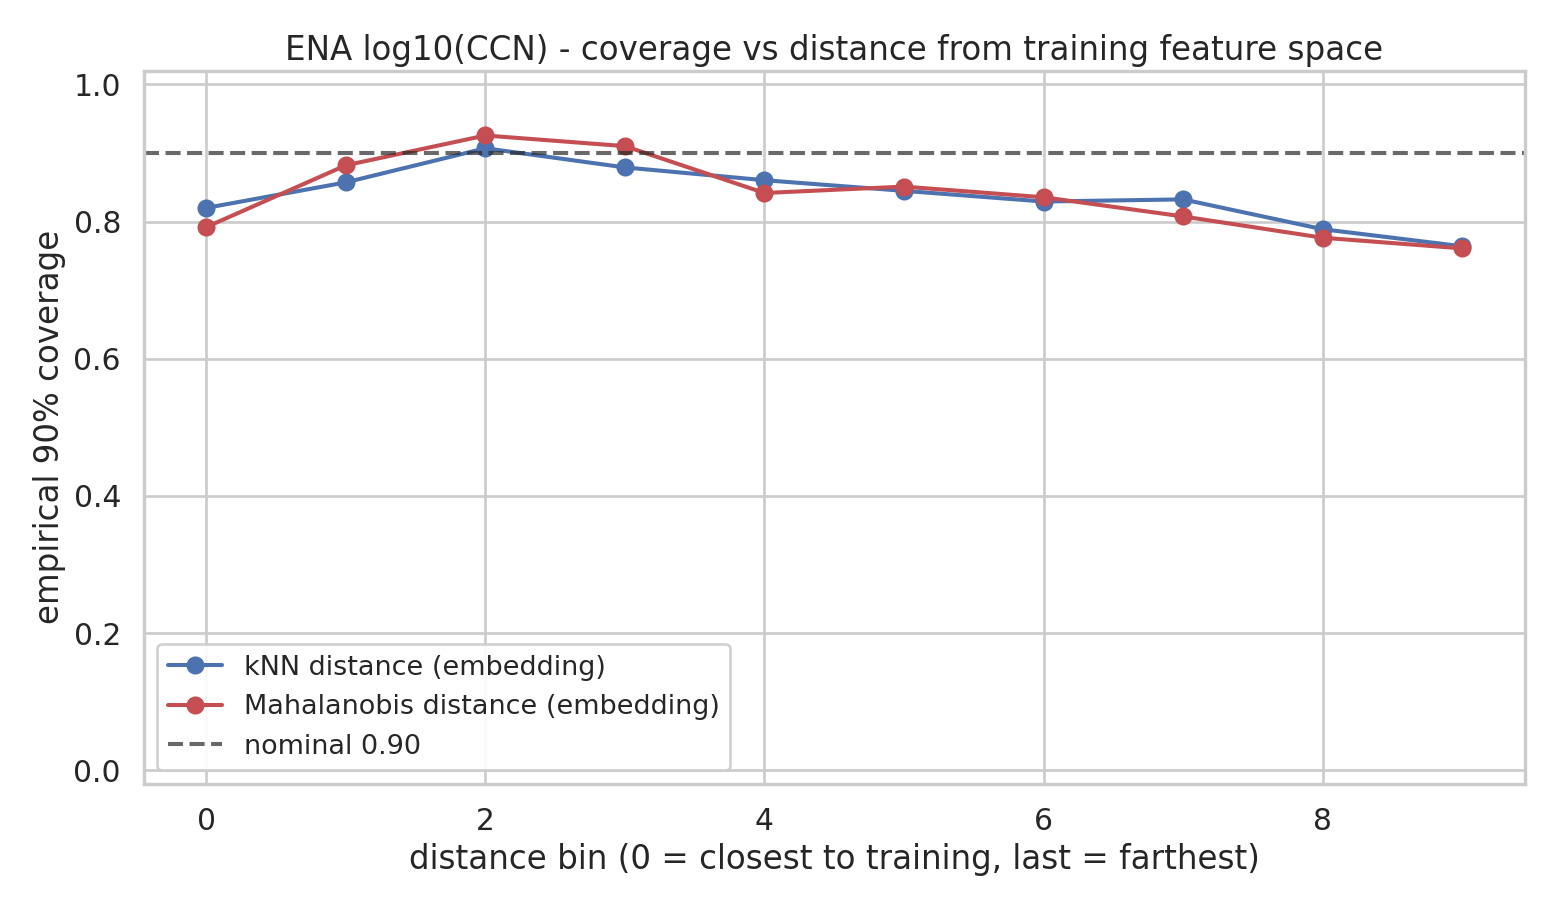
\includegraphics[width=\textwidth]{fig_preadd_oos.png}
    \\[-0.2em]{\small \textbf{Pre-additive} (hidden 128)}
  \end{minipage}\hfill
  \begin{minipage}{0.49\textwidth}\centering
    \fbox{\parbox[c][3.0cm][c]{0.9\textwidth}{\centering\small \textbf{Vanilla (flat)}: N/A\\no learned embedding; raw
    $5302$-d distance is degenerate, so this diagnostic does not apply}}
    \\[-0.2em]{\small \textbf{Vanilla (flat)}}
  \end{minipage}
  \caption{Coverage vs.\ distance from training (in the model's LSTM embedding
  space), $k$NN and Mahalanobis, for each architecture's best run. The LSTM heads
  stay roughly flat (paper split is in-distribution). The flat \emph{vanilla} model
  has no learned embedding, so the diagnostic does not apply.}
  \label{fig:oos}
\end{figure}

\medskip
\noindent
\textbf{Caveat.} The paper split is in-distribution, so a flat curve is expected and
is \emph{not} evidence of extrapolation. An out-of-support split (high-CCN tail
\texttt{ccn\_tail}, or a shifted \texttt{event}) is the real test; not yet run.

\end{document}
